\documentclass[11pt,a4paper]{article}
\usepackage[utf8]{inputenc}\usepackage[T1]{fontenc}
\usepackage[margin=1in]{geometry}
\usepackage{amsmath,amssymb,booktabs,graphicx,enumitem,xcolor,parskip,titlesec,multirow}
\usepackage[hidelinks]{hyperref}
\graphicspath{{figures/}}
\definecolor{qnavy}{RGB}{20,40,75}\definecolor{qgrey}{RGB}{90,90,90}\definecolor{qred}{RGB}{150,30,30}
\titleformat{\section}{\large\bfseries\color{qnavy}}{\thesection}{0.6em}{}
\begin{document}\thispagestyle{empty}
\noindent
{\large\bfseries\color{qnavy} Report R04 --- Glioma Molecular Epidemiology and Prognosis}\\[2pt]
{\color{qgrey}Two cohorts, $\sim$2{,}000 patients, no imaging. Includes a correction to the
comparison with R02.}\\[6pt]
{\color{qgrey}\rule{\textwidth}{0.4pt}}

\medskip
\noindent 7 August 2026 \quad\textbullet\quad Quantara

\section*{Summary}

Across TCGA pan-glioma ($n=1{,}040$ with survival) and the MSK panel cohort ($n=923$), the
molecular markers behave exactly as established biology predicts, and the pipeline recovers
them at overwhelming significance. IDH mutation carries a median survival of 89.7 months
versus 14.0 for wild-type ($p=5.7\times10^{-71}$). The three-tier CNS5 subtype
stratification separates cleanly: codeleted 115.8 months, non-codeleted 75.1, IDH-wildtype
14.0 ($p=2.3\times10^{-70}$).

\textbf{The headline finding is a correction, not a claim.} A naive reading of these data
says the molecular panel (C-index 0.797) far outperforms imaging (0.602 in R02). \emph{That
comparison is invalid}, and the audit caught it before this report was written. TCGA spans
grades 2--4 while UPENN-GBM is glioblastoma only, and IDH status largely \emph{is} the
grade distinction. Restricting TCGA to glioblastoma --- the like-for-like comparison ---
the molecular panel collapses to \textbf{0.541--0.561}, below the \textbf{0.602} that
imaging achieved.

\section{Results}

\subsection*{Positive control and stratification}

\begin{center}
\begin{tabular}{@{}lrrr@{}}
\toprule
\textbf{Group} & \textbf{$n$} & \textbf{Median OS (months)} & \textbf{Test} \\
\midrule
IDH mutant & \multirow{2}{*}{919} & 89.7 & \multirow{2}{*}{$p=5.7\times10^{-71}$} \\
IDH wild-type & & 14.0 & \\
\midrule
IDHmut-codeleted & 151 & 115.8 & \multirow{3}{*}{$p=2.3\times10^{-70}$} \\
IDHmut-non-codeleted & 247 & 75.1 & \\
IDH wild-type & 503 & 14.0 & \\
\bottomrule
\end{tabular}
\end{center}

\begin{center}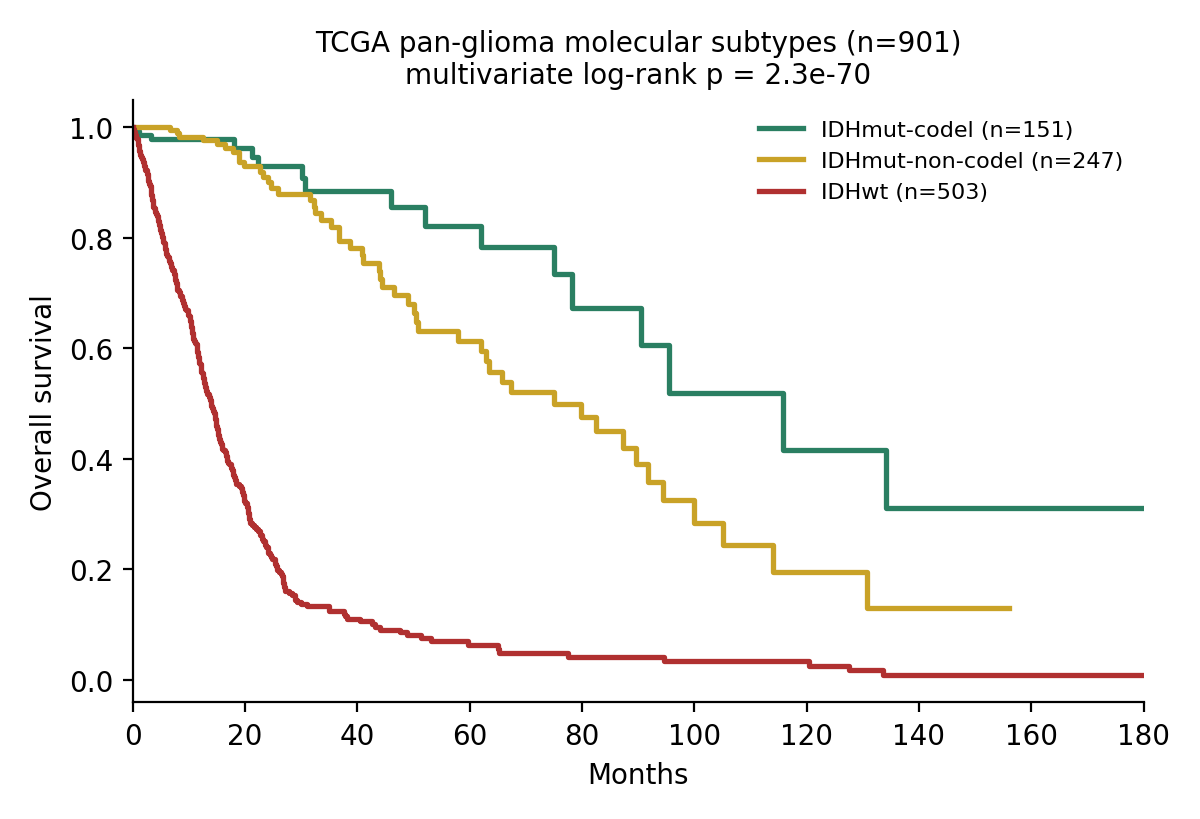
\includegraphics[width=0.62\textwidth]{fig1_km_subtypes.png}\end{center}

\subsection*{Marker co-occurrence --- the CNS5 variables are not independent}

\begin{center}
\begin{tabular}{@{}lrrrl@{}}
\toprule
\textbf{Pair} & \textbf{Odds ratio} & \textbf{$p$} & \textbf{$q$ (BH)} & \textbf{Reading} \\
\midrule
IDH $\times$ TERT promoter & 0.186 & $7.6\times10^{-10}$ & $1.1\times10^{-9}$ & mutually exclusive \\
IDH $\times$ MGMT & 17.11 & $3.5\times10^{-58}$ & $1.1\times10^{-57}$ & strongly co-occurring \\
TERT $\times$ MGMT & 1.05 & 0.89 & 0.89 & independent \\
\bottomrule
\end{tabular}
\end{center}

\noindent
Both non-null results match known biology: IDH-mutant and TERT-promoter-mutant tumours use
largely alternative routes, and IDH-mutant gliomas are overwhelmingly MGMT-methylated (the
G-CIMP phenotype). This is a second, independent confirmation that the data and joins are
sound.

\subsection*{Independent replication in the MSK cohort ($n=923$)}

\begin{center}
\begin{tabular}{@{}lrrrr@{}}
\toprule
\textbf{Marker} & \textbf{$n$ positive} & \textbf{HR} & \textbf{$p$} & \textbf{C-index} \\
\midrule
TERT promoter mutation & 548 & 1.69 & $2.8\times10^{-6}$ & 0.591 \\
CDKN2A homozygous deletion & 283 & 2.37 & $4.3\times10^{-14}$ & 0.588 \\
Both & --- & --- & --- & 0.627 \\
\bottomrule
\end{tabular}
\end{center}

\section{\textcolor{qred}{The correction: prognostic performance tracks grade mix, not marker panel}}

\begin{center}
\begin{tabular}{@{}lccc@{}}
\toprule
\textbf{Predictor} & \textbf{TCGA all grades} & \textbf{Glioblastoma only} & \textbf{$n$ (GBM)} \\
\midrule
IDH only & 0.719 & \textbf{0.541} & 470 \\
IDH $+$ MGMT & 0.747 & \textbf{0.561} & 356 \\
IDH $+$ MGMT $+$ TERT & 0.797 & not estimable & 26 \\
\midrule
\textbf{Imaging alone (R02, UPENN-GBM)} & --- & \textbf{0.602} & 574 \\
\bottomrule
\end{tabular}
\end{center}

\begin{center}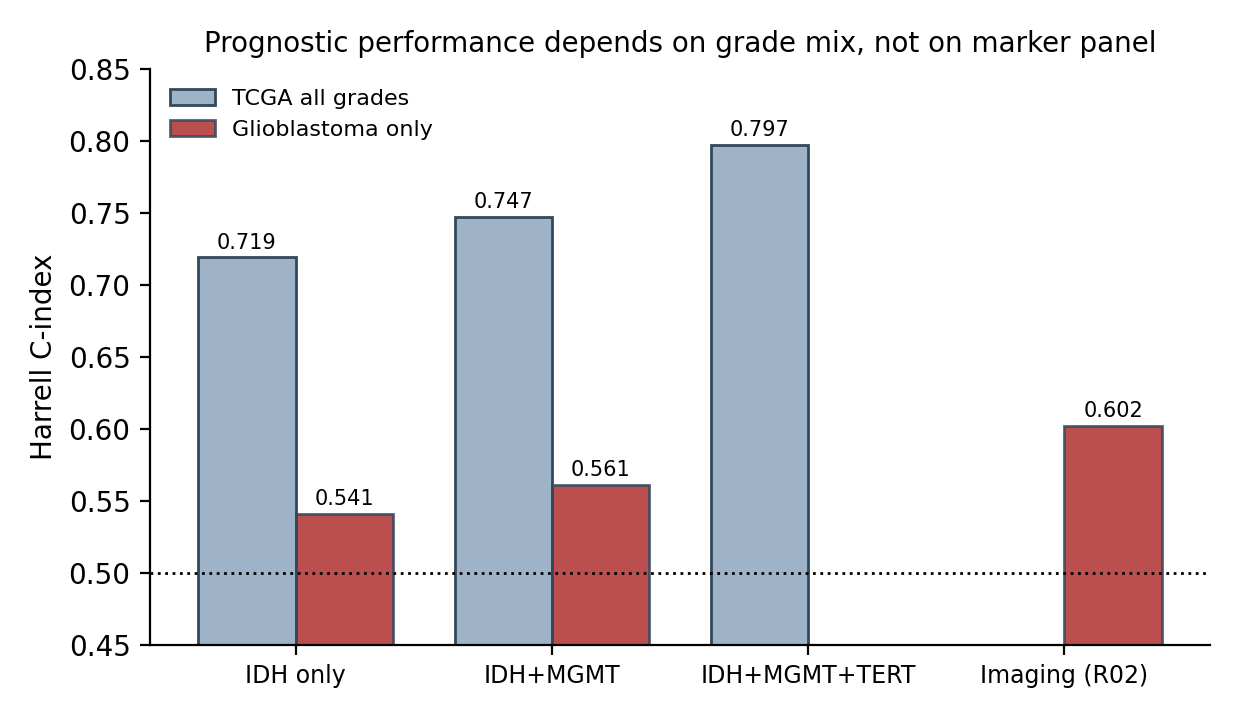
\includegraphics[width=0.76\textwidth]{fig2_cindex_comparison.png}\end{center}

\noindent
\textbf{Within glioblastoma, the standard molecular panel carries little prognostic
information (0.541--0.561) while imaging carries more (0.602).} The panel's apparent
strength across all grades is real but largely tautological: IDH status is close to a proxy
for whether the tumour is a low-grade glioma or a glioblastoma, and that distinction
dominates survival.

Cross-validation optimism was also checked and is modest --- 0.719 falls to 0.707 and 0.797
to 0.759 under 5-fold CV --- so it is the cohort composition, not overfitting, that drives
the difference.

\section{What R02 and R04 say together}

\begin{enumerate}[leftmargin=1.6em,nosep]
\item Molecular markers are outstanding at separating glioma \emph{types} and therefore
survival across grades. Nothing here challenges that.
\item Within glioblastoma specifically, they add little prognostically --- and imaging adds
more.
\item R02 showed the imaging signal is independent of age ($p=1.6\times10^{-9}$). R04 now
shows it is also not simply recapitulating the molecular panel, because that panel performs
worse in the same disease setting.
\item R01 remains consistent: imaging does not encode MGMT status, and MGMT itself adds
essentially nothing within glioblastoma (0.719 $\to$ 0.747 across grades, 0.541 $\to$ 0.561
within GBM).
\end{enumerate}

\noindent
That is a coherent, defensible position for the glioma arm: \textbf{imaging is worth
studying prognostically in glioblastoma precisely because the molecular panel is weak
there}.

\section{Limitations}

\begin{itemize}[leftmargin=1.4em,nosep]
\item The imaging and molecular results come from \emph{different cohorts} (UPENN-GBM vs
TCGA). They are matched on disease but not on population, treatment era or follow-up. A
within-cohort head-to-head would need molecular markers on the UPENN patients --- IDH1 and
MGMT are available there and this is the obvious next analysis.
\item TERT is available on only 311 TCGA patients and just 26 glioblastomas, so the
three-marker panel cannot be evaluated within GBM at all.
\item C-indices for the panels are from Cox models on binary markers, not a tuned learner.
\item TCGA treatment is heterogeneous and pre-dates current standards.
\end{itemize}

\section{Audit}

\begin{center}
\begin{tabular}{@{}llp{7.2cm}@{}}
\toprule
\textbf{Check} & \textbf{Verdict} & \textbf{Finding} \\
\midrule
Positive control & \textbf{Recovered} & IDH $p=5.7\times10^{-71}$, correct direction \\
Cohort comparability & \textbf{FAILED as first framed} & TCGA spans grades 2--4; UPENN is GBM only. Comparison corrected in \S3 \\
CV optimism & \textbf{Modest} & 0.719$\to$0.707; 0.797$\to$0.759 \\
Co-occurrence sanity & \textbf{Matches biology} & IDH/TERT exclusive, IDH/MGMT co-occurring \\
Independent replication & \textbf{Yes} & TERT and CDKN2A both prognostic in MSK, $n=923$ \\
Gates & \textbf{4 / 4 PASS} & After one documented failure, see below \\
\bottomrule
\end{tabular}
\end{center}

\noindent
A gate failed on the first attempt: expected 1{,}046 survival records, observed 1{,}040. Six
patients have \texttt{OS\_MONTHS} $=0$, which a Cox model cannot use. The expectation was
too tight; it was corrected to 1{,}040 with the reason recorded in source, and the failed
run is retained as \texttt{gates\_FAILED\_first\_attempt.json}.

\section{How to verify}

\texttt{evidence/} contains \texttt{config.yaml} (hash \texttt{18ea8aa0\ldots}, written
before any outcome was read), \texttt{gates.json}, the failed run's gates,
\texttt{results.json} with every statistic, \texttt{tcga\_survival.csv},
\texttt{inputs.json} (file hashes), \texttt{MANIFEST.sha256}, \texttt{env.txt}, and both
scripts.

\vfill
\noindent{\color{qgrey}\rule{\textwidth}{0.4pt}}\\
{\footnotesize\color{qgrey}Run \texttt{runs/20260806T235340Z-R04glioma-3f8bece}. Data:
cBioPortal \texttt{lgggbm\_tcga\_pub} (Broad GDAC/NIH terms) and
\texttt{glioma\_mskcc\_2019} (ODbL). No patient-level identifiers reproduced.}
\end{document}
